% Integration by parts as a rectangle cut by a graph. f(0)=0.
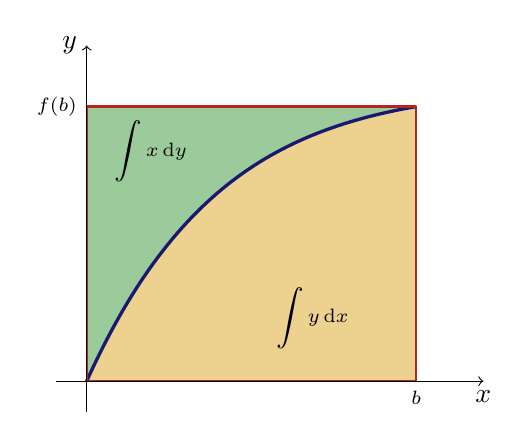
\begin{tikzpicture}[x=1.55cm,y=1.55cm,line join=round]
  \fill[Goldenrod!50] (0,0) .. controls (0.7,1.55) and (1.55,2.05) .. (2.7,2.25) -- (2.7,0) -- cycle;
  \fill[ForestGreen!45] (0,0) .. controls (0.7,1.55) and (1.55,2.05) .. (2.7,2.25) -- (0,2.25) -- cycle;
  \draw[MidnightBlue,very thick] (0,0) .. controls (0.7,1.55) and (1.55,2.05) .. (2.7,2.25);
  \draw[BrickRed,thick] (0,0) rectangle (2.7,2.25);
  \draw[->] (-0.25,0) -- (3.25,0) node[below] {$x$};
  \draw[->] (0,-0.25) -- (0,2.75) node[left] {$y$};
  \node[font=\scriptsize,anchor=north] at (1.85,0.85) {$\displaystyle\int y\,\mathrm{d}x$};
  \node[font=\scriptsize,anchor=south west] at (0.15,1.55) {$\displaystyle\int x\,\mathrm{d}y$};
  \node[font=\scriptsize,below] at (2.7,0) {$b$};
  \node[font=\scriptsize,left] at (0,2.25) {$f(b)$};
\end{tikzpicture}
